
% this file is called up by thesis.tex



\chapter{Material \& metoder} % top level followed by section, subsection
\label{ch:metoder}

% ----------------------- paths to graphics ------------------------

% change according to folder and file names
\ifpdf
    \graphicspath{{8/figures/PNG/}{8_materials_and_methods/figures/PDF/}{8_materials_and_methods/figures/}}
\else
    \graphicspath{{8/figures/EPS/}{8_materials_and_methods/figures/}}
\fi

% ----------------------- contents from here ------------------------



\section{Metoder}
Nu när gruppen hade ett problem återstod det att lösa problemet. I kittet fanns olika komponenter och sensorer. I början var uppmärksamheten riktad mot en vibrationssensor för att upptäcka slag eller skadegörelse mot glasrutorna, dock visade det sig omedelbart att den var för känslig. Under tiden var det bestämt att använda en pir-sensor som skulle upptäcka rörelse inne i hållplatsen och därefter tända en lampa en viss period av tid. Tanken var att göra väntande busspassagerare trygga med hjälp av ljuset medan de väntade på bussen. Tillbaka till skadegörelsen av glasrutorna för att nu hade gruppen bestämt sig för att använda en ljud-sensor för att upptäcka slag eller skadegörelse mot en glasruta. En IP-kamera var installerad i mitten av vägen för att först filma hållplatsen och även runt omkring i ett varv om 360 grader. 
För att hela systemet skulle kunna fungera samtidigt så användes en schemaläggare så att varje komponent kunde vara aktiv utan att begränsa andra komponenter. Detta var nödvändigt att göra eftersom sensorer som användes skulle lyssna kontinuerligt på förändringar hos omgivningen medan systemet var aktivt och utförde andra uppgifter.\\

Pir-sensorns uppgift var att lysa upp busshållplatsen vid rörelse i den. Ljud-sensorns uppgift var att tala om för mikroprocessorn att aktivera IP-kameran så den filmade och skickade iväg filmen till en server. Därför upprättades en FTP-server för att kunna ta emot inspelningar och olika data från kameran och lagra dessa på en dator. Det behövdes ett nätverk för att åstadkomma kommunikation mellan de olika delarna. Mikroprocessorn med sina sensorer tillsammans med kameran och FTP-servern var uppkopplade inom samma nät, delvis via WIFI-anslutning och delvis med direkt-kabel-anslutning.

De finns olika task  i systemet som exekveras parallellt för att kunna låta processorn jobba med flera saker samtidigt. Det finns totalt 3 tasks i systemet varvid två av de (pirsensorn och ljudsensorn) agerar som input till systemet. Den tredje tasken (WifiTask) kontrollerar om det finns en wifi-anslutning, om anslutningen är nere försöker den återansluta till wifi.
Biblioteket som möjliggör att dessa tasks arbetar oberoende av varandra och som detta systemet använde sig av skapades av Nicholas Wiersma och heter ESP8266Scheduler. 
\\


\section{ESP8266 - mikroprocessorn}
Huvudanledningen för valet av denna mikroprocessor var att den hade en inbyggd Wifi-mottagare vilket var absolut nödvändigt för att kunna kommunicera med nätverket där kameran var uppkopplad. Givetvis kunde gruppen hitta på alternativa lösningar men just denna lösning var den smidigaste. I övrigt fanns det allt de behövde till deras projekt. Det fanns gott om digitala pins samt en analog-pin, dock tog den emot max 1 V. \\

Deras tanke var att kopppla sensorer till ESP:n som sedan kommunicerade med kameran utifrån de uppgiffter som lästes in från sensorerna. ESP:n var då kopplad till samma nätverk som kameran och kommunicerade och skickade kommandon till kameran.\\
\section{FTP-Server}
För att kunna identifiera personer som ligger bakom skadegörelser behövde systemet lagra bilder eller/och filmer på en server och den var en viktig del av lösningen. Gruppen valde att använda en FTP-server där bilder och/eller filmer skulle lagras. FTP-servern låg under samma subnät som IP-kameran. Information om FTP-servern:

\begin{itemize}
\item IP adress : 192.168.0.106

\item Port nummer : 21

\item Användarnamn : ”FTP-User”

\item Lösenord : ”Safe24”

\end{itemize}
\section{IP-kameran}
Kameran som används var tillhandahållen av AXIS. Kameran var en Q6128-E Network Camera med möjlighet till att via  internetuppkoppling sända bilder och streama video till en server.\\

IP-kameran användes för att skicka bilder och video till en server för datalagring.

Kommunikationen med kameran gjordes via ESP8266 som sände kommandon över internet för att styra kameran.

Grupperna skapade tre aktiviteter i kameran, ”ActionPTZStation1”, ”ActionRecord”, ”ActionPTZHome”.
ActionRecord var en aktivitet som spelade in en film som var en minut lång och skickade den till FTP-server som har namnet FTP-Safe24. Filmens upplösning som skickades till FTP-servern var 3840x2860. Ett suffix lades i filmen som innehöll datum och tidsinformation. ActionRecord aktiverades när virtuell port 9 var aktiv.\\
ActionPTZHome var den som riktade kameran till hemposition. Kamerans hemposition var definierad som position ”Safe24”. ActionPTZHome kunde aktiveras genom att aktivera virtuell port nummer 10.
ActionPTZStation1 var den som riktade kameran till position som heter ”plats1” (busshållplatsen). ”. ActionPTZHome kunde aktiveras egenom att aktivera virtuell port nummer 8.


\section{Sensorer}
En PIR-sensor från Adafruit användes som rörelsedetektor för att lysa upp den stora lampan. Den kopplades till ESP:n via tre sladdar, en röd som gick till strömmen, trots att det krävdes minst 5 V så gick det bra med 3,3 V från ESP:n. Den andra sladden gick till jord och den tredje är själva signalsladden som då gick till en digital pin som var satt till input-mode. För att gruppen skulle lyckas med pir-sensorn fick de med hjälp av delay och en counter räkna in hur många gånger som signalen är hög eller låg. Efter flera tester och försök kom de fram till att det behövdes minst 7 rundor där en runda är på 0,5 s. Anledningen till detta var att näär det inte fanns rörelse så gav PIR-sensor utsalg med 6 ettor och en nolla. Då det fanns rörelse gav den utslag på bara ettor. Slutligen gällde det att om programmmet läste in 7 värden från signal-pin, så skulle summan vara 7 vid rörelse och om summan var under sju betydde det att ett av värden var noll, alltså ingen rörelse. Ibland kom det även störningar som gjorde att PIR-sensorn bara visade ettor, vilket senare fram i tiden löstes genom att utföra en digitalWrite på PIR-input-pin:n med värdet låg.  \\

\begin{figure}[h]

  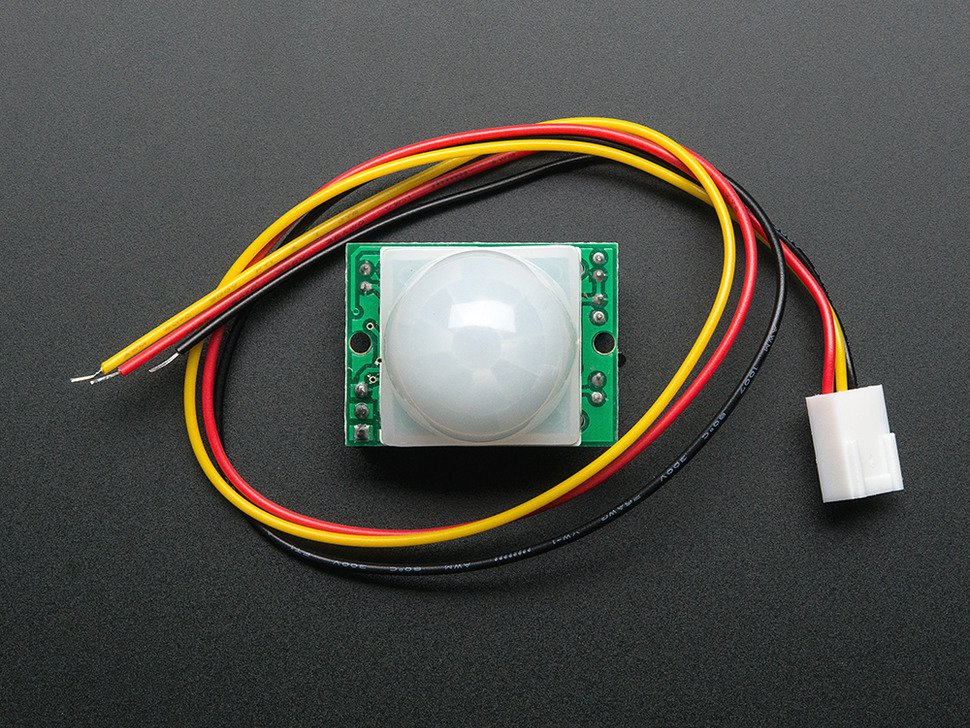
\includegraphics[width=\linewidth]{pir.jpg}
  \caption{En PIR-sensor från Adafruit. (www.adafruit.com)}
  \label{fig:pir}
\end{figure}
PIR-sensorn registrerade ifall det förekom någon rörelse. Denna sensorn skickade digitala värden till ESP8266.\\

På grund av vibrationssensorn var så känslig använde gruppen en ljudsensor istället som hade mikrofon. På samma sätt som PIR-sensor kopplades den till ström och jord och en tredje sladd gick till analog-pin istället för en digital. Eftersom en digital pin gav antingen en låg eller hög signal, dvs antingen en etta eller en nolla, medan den analoga pin:n gav olika heltals-väärden beroende på styrkan av signalen, som egentligen motsvarade för högre spänning. 
Glas har så som andra material en naturlig resonansfrekvens med vilken material oscillerar eller enklare sagt vibrerar. Självklart varierar denna frekvens från typ till annan beroende av glasets form och om det innehåller något dämpande. Ljud som har samma ton som den naturliga frekvensen kan få glas att börja vibrera. Det krävs även en hel del ”styrka” vid sidan av tonen. Ju högre ljudet är desto mer vibrerar glaset, och vid en viss gräns kommer inte glaset att tåla dessa vibrationer och därför går glaset i sönder. Det krävs att man kommer upp till över 100 dB. Det säger egentligen inte mycket, om man inte vet i förväg att en människas normala tal är runtomkring 50 dB. 

På grund av brist på glas och utrymme för gruppen för att de skulle  göra försök att ta i sönder glas hade de bestämt i detta projekt att utgå från slag mot en kartong eller en miniatyr av en hållplats med en gräns på 75 dB. Över denna gräns betydde det att de har glas som hade gått i sönder.\\
\begin{figure}[h]

  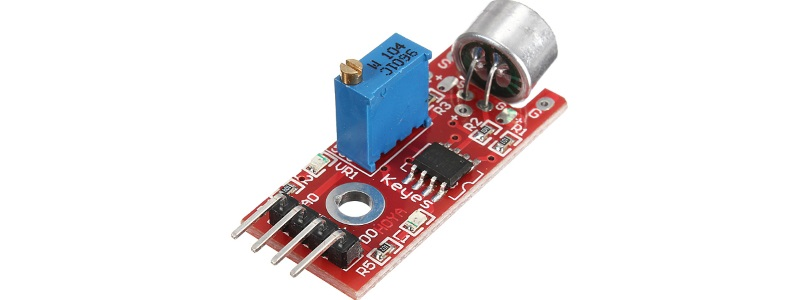
\includegraphics[width=\linewidth]{mic.jpg}
  \caption{En ljudsensor med mikrofon. (www.bazaargadgets.com)}
  \label{fig:mic}
\end{figure}

\section{Arbetsuppgifter}
Gruppen arbetade både tillsammans och även enskilt så att var och en av gruppmedlemmarna kunde bidra med något. Benjamin var delaktig i arbetet med flödesdiagram, tasks, hjälp med byggandet av busshållplats och även testfall. Yurdaer arbetade med wifi-kodning av ESP:n, kamera-kommandon, ftp-servern och i rapporten skrev han om sina delar samt om etiska aspekter. Georges bidrag var med struktur av kod, API, manual, testfall, FTP-servern och en del rapportskrivning. Han bidrog även med upprättande av en Latex-mall för rapporten. Louay arbetade med sensorernas kodning, ihopkoppling av alla komponenter, förslag till router-lösning, byggandet av en hållplats och kontinuerlig testning av alla kopplingar. 
% ---------------------------------------------------------------------------
%: ----------------------- end of thesis sub-document ------------------------
% ---------------------------------------------------------------------------



 



